\documentclass[10pt,twocolumn,letterpaper]{article}

\usepackage{cvpr}
\usepackage{times}
\usepackage{epsfig}
\usepackage{graphicx}
\usepackage{amsmath}
\usepackage{amssymb}
\usepackage{float}
\usepackage{multicol}
\usepackage{lipsum}
\usepackage{booktabs}

%\usepackage{rotating}
% Include other packages here, before hyperref.

% If you comment hyperref and then uncomment it, you should delete
% egpaper.aux before re-running latex.  (Or just hit 'q' on the first latex
% run, let it finish, and you should be clear).
\usepackage[pagebackref=true,breaklinks=true,letterpaper=true,colorlinks,bookmarks=false]{hyperref}

\cvprfinalcopy % *** Uncomment this line for the final submission

\def\cvprPaperID{****} % *** Enter the CVPR Paper ID here
\def\httilde{\mbox{\tt\raisebox{-.5ex}{\symbol{126}}}}

% Pages are numbered in submission mode, and unnumbered in camera-ready
\ifcvprfinal\pagestyle{empty}\fi
\begin{document}

%-----------------------------------------------------------------------------------------------------------------------
% -- title
%-----------------------------------------------------------------------------------------------------------------------

\title{
CS 7643 - Deep Learning \\
Image Captioning with Deep Learning \\
}

%-----------------------------------------------------------------------------------------------------------------------
% -- authors
%-----------------------------------------------------------------------------------------------------------------------

\author{
Christoper Dugan, Mouhcine Aitounejjar, Walker Stevens, Xuan Xu\\
Georgia Institute of Technology\\
{\tt\small {\{cdugan3, maitounejjar3, wstevens36, xuanxu\}}@gatech.edu}
}

\maketitle
%\thispagestyle{empty}

%-----------------------------------------------------------------------------------------------------------------------
% -- abstract
%-----------------------------------------------------------------------------------------------------------------------

\begin{abstract}
   With an estimated 250 million blind or visually impaired people in the world, the task of image captioning is an important one that has seen much success in the past decade. Image captioning models are typically evaluated using scores like CIDEr or BLEU-4, which evaluate the accuracy of a generated caption against the ground truth label. In this paper, our team implemented two of these image captioning models and evaluated their performance using not only BLEU-4, but also with captioning visualizations that demonstrate the inner workings of each model. In addition to these evaluations, the team explored knowledge distillation as a potential tool to reduce the size of image captioning models while retaining good performance.
\end{abstract}


%-----------------------------------------------------------------------------------------------------------------------
\section{Introduction / Background / Motivation}
%-----------------------------------------------------------------------------------------------------------------------
% NOTE -- we expect about 2 pages out of this section
Image captioning is a computer vision task, in which deep neural networks are trained to automatically generate meaningful natural language sentences that describe what is taking place in an input image. This task lies at the intersection of two sub-domains in machine learning: natural language processing (NLP) and image processing.

Image captioning has numerous applications in real life, of which the most noble and humane is the potential for a substantial quality of life improvement for millions of people who suffer from various degrees of visual impairment. Other application fields include image indexing and search, social media and medical sciences.\\

\subsection{Image Captioning Visualizations}
In the first part of this project, we aimed to tackle the explainability portion of image captioning, by trying to understand why a model captions an image in a certain way. One way to approach this is by plotting the attention during inference. In simplistic terms, this can be thought of as the image captioning equivalent of the saliency maps and Grad-CAM heatmaps that we experimented with in Assignment 3 in this course (\cite{zeiler2014visualizing}, \cite{simonyan2013deep} and \cite{selvaraju2017grad}). We essentially  want to capture and visualize what the model considered when it generates words describing an image. Explainability continues to gain traction in deep learning research, as a way to understand why models make the decisions they make. It also helps build trust in ML models, uncover biases and understand failure modes. A visualization of this nature typically shows a heatmap overlaid on the original image, showing which parts of the image were most influential in choosing that particular word as part of the caption.

Some of the earliest image captioning models, such as the \textit{"Show, Attend and Tell"} paper \cite{xu2015show} used visualization tools to demonstrate that their new attention-based image captioning technique was focusing on the correct part of the image for each word in the caption. Similar analysis was performed in \cite{cornia2022explaining} where the authors used visualization as a support of their quantitative results to analyze transformer-based image captioning models. Oftentimes, however, models are only evaluated quantitatively using the BLEU-4 or similar metrics. We can use the scores from these evaluations to sort models based on their BLEU-4 score and decide which is the “best” model overall, shown in Figure \ref{fig:COCOBest}. But, this evaluation doesn’t reveal the “how” of model performance. That is where visualizations can help us do a more nuanced analysis than the current research does.

In particular, we would like to compare different image captioning models and use visualizations to justify their performance. For example, if image captioning model A scores a higher BLEU-4 score than model B, we would like to take visualizations of the captions for each of these models on the same images and compare them directly to try to understand why model A performs better. With this methodology, we hope to gain insight into how to improve models when they’re underperforming or to understand why a model might not be performing as we expect it to.

In our quest to better understand image captioning models, we will focus on existing state-of-the-art image captioning models. One such state-of-the-art model is BLIP \cite{blip2022}, which effectively transfers to both vision-language understanding and generation tasks. BLIP addresses some of the limitations of existing pre-trained models by utilizing noisy web data through a process called bootstrapping captions. A captioner generates synthetic captions, and a filter removes the noisy ones, which helps the model to better learn from the available data. BLIP has achieved state-of-the-art results on several vision-language tasks, such as image-text retrieval, image captioning, and visual question answering, demonstrating its strong generalization ability. In our project, we plan to employ BLIP for image captioning and compare its performance to other models. By understanding the differences in the attention mechanisms and visualizations between our models and BLIP, we hope to gain insights into how we can further improve our models and their performance on the image captioning task.

Improved image captioning model visualizations are a step towards making improved models that have better and faster performance. Firstly, visualizations can help us understand instances where the model is behaving unexpectedly. We can use that as a starting point for our improvements, either by modifying and augmenting data to train the model to better handle these instances or by modifying model architecture to better handle these instances. Secondly, visualizations serve as a valuable method of qualitative comparison for comparing models. For instance, if one model performs better than another, we can study the models’ visualizations side-by-side to identify where the worse model is falling short and then take action to improve it. These applications are both examples of where our image captioning model visualizations can help to improve our understanding of image captioning and ultimately improve these models’ performance.

\begin{figure}[t]
\begin{center}
   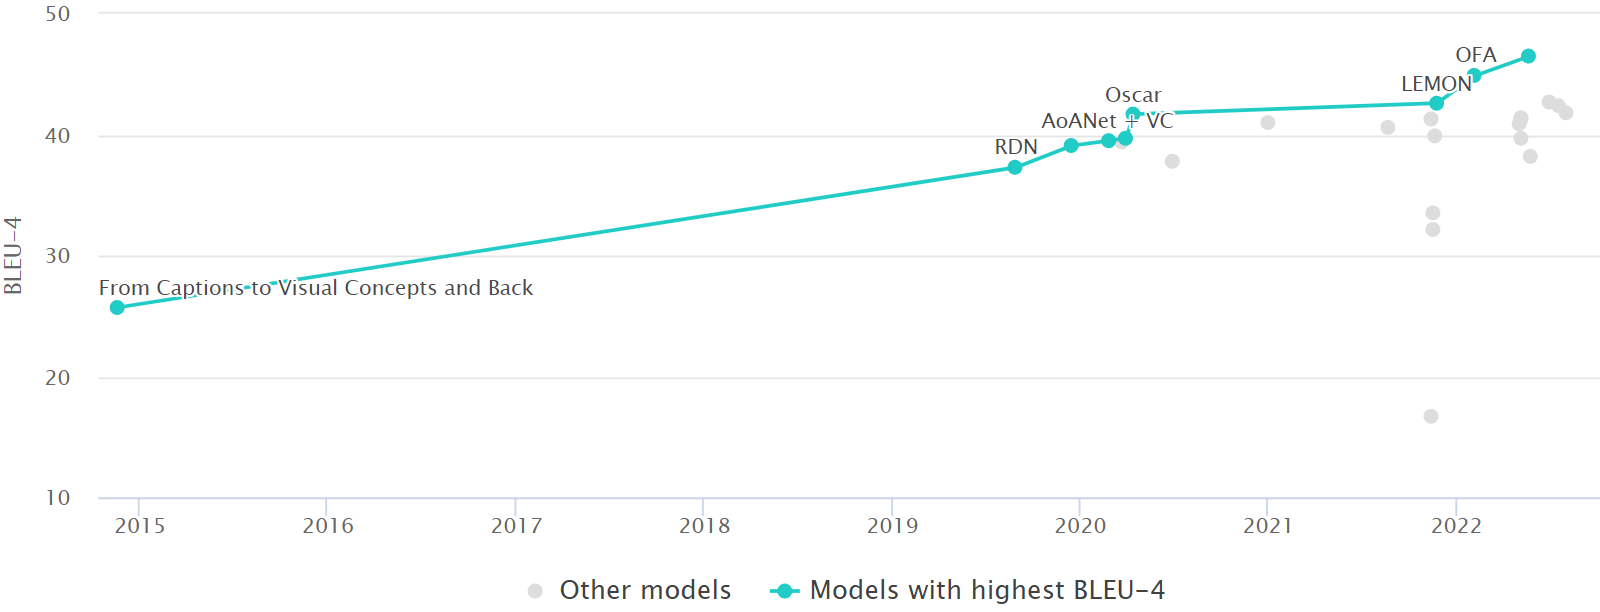
\includegraphics[width=1.0\linewidth]{images/COCO_Image_Captioning_Scores.png}
\end{center}
   \caption{Image Captioning Models Ranked by BLEU-4 Scores on COCO Dataset - \href{https://paperswithcode.com/sota/image-captioning-on-coco-captions}{link}}
\label{fig:COCOBest}
\end{figure}

\subsection{Knowledge Distillation with Image Captioning}
While it is necessary to train a large multimodal model to capture nuanced features, oftentimes it is not efficient to deploy a large model in standard devices. For example, running large models could require a challenging setup. Knowledge distillation (KD) can effectively compress the redundant representation learnt in the large teacher model and allow the student model to reach almost the same result as the teacher model. Therefore, in addition to visualizing our image captioning models, we would like to explore KD as a method of maintaining model performance while reducing model size. We adopted the word-level KD method demonstrated by Kim et al. \cite{kim2016sequencelevel} to distill a larger sequence-to-sequence model with attention, ResNet101-LSTM(512 hidden), into a smaller model, ResNet50-LSTM(256-hidden). The goal is to compress the somewhat cumbersome teacher model by transferring the "dark knowledge" learnt by a sophisticated teacher model to a simpler student model. We also hope to understand the KD algorithm, by experimenting with different temperature values and KD loss weights.

KD was initially formulated by Hinton et al. \cite{hinton2015distilling}. Since its introduction, KD has evolved to use distillation from logits (\cite{cho2019efficacy},\cite{furlanello2018born}), features (\cite{heo2019comprehensive},\cite{park2019relational}) and attention \cite{zagoruyko2017paying}. For sequence-to-sequence or generative models, Kim et al. \cite{kim2016sequencelevel} adapted KD to neural machine translation by introducing the concept of sequence-level distillation, where the student is trained on the output from the beam search of the teacher network that had the highest similarity with the target sequence. In our experiments, we distilled both knowledge from the feature output of the ResNet encoder and word-level softened probability distribution from the LSTM decoder. By tuning the temperature of probability distribution, we hope to understand the KD loss function and successfuly distill a lightweight student model.

\subsection{Dataset Information}

For this project, the team chose to use the Microsoft Common Objects in Context (MS COCO or COCO) \cite{lin2014microsoft} dataset because of its convenience for training image captioning models and its widespread popularity in this field. This dataset contains 123,000 images, each with 5 independent human-generated captions. Our experiments used the recommended training/validation split of 118K/5K images. The images were first compiled in February 2014 by a team from Microsoft and contain "complex everyday scenes containing common objects in their natural context". The original purpose of these images was for object recognition, so the images were collected by searching for certain objects on the website Flickr, a repository of photos uploaded by amateur photographers. In April 2015 \cite{chen2015COCOCaptions} the dataset was expanded by another Microsoft team to include captions of these images, to help train image captioning models. For the captioning, human subjects were asked to "describe all the important parts of the scene" with at least 8 words. In addition to MS COCO, we also used the Flickr 8k dataset as a testing set to compare our models because of its convenient small size. It has similar properties to MS COCO but contains only 8,000 images.

Because the datasets contain only photos, the trained models may struggle with images that are not photos (such as cartoons or paintings). Also, because the captions do not contain proper names (names of important people, places, or companies), the models will not recognize particular places or famous people. However, the dataset is ideal for training image captioning models for everyday usage, for example as an aid to visually-impaired people.

%-----------------------------------------------------------------------------------------------------------------------
\section{Approach}
%-----------------------------------------------------------------------------------------------------------------------
% NOTE -- we expect about 1 page out of this section

\subsection{Image Captioning Visualizations}\label{sec:blipapproach}

To better understand the attention mechanisms and decision-making processes of state-of-the-art models, we decided to explore the image-captioning model, BLIP \cite{blip2022}. Our goal was to analyze the attention mechanism of BLIP through Grad-CAM visualizations and compare it the attention mechanism of Resnet101-LSTM.

To implement BLIP in our project, we first obtained the pre-trained BLIP model, fine-tuned on COCO specifically for image captioning tasks \cite{lavis2022}. We preprocessed the images from the Flickr8k dataset to be compatible with the BLIP model input format, and then generated image captions using the BLIP model.

We employed Grad-CAM visualization techniques to visualize the attention mechanism of BLIP when generating captions. For our visualizations, we used the Flickr8k dataset, as it provided a diverse set of images with varying complexity. This allowed us to better analyze the model's attention mechanism and decision-making process, given it was unseen data.

Comparing the Grad-CAM visualizations of BLIP with Resnet101-LSTM, we analyzed the differences in their attention mechanisms and decision processes. Our goal was to identify areas of improvement for our models by gaining insights into the model's performance and decision-making process, ultimately enhancing their adeptness at image captioning.

\subsection{Knowledge Distillation}
To explore knowledge distillation for image captioning, we started with the pre-trained ResNet101-LSTM with attention as the teacher model, from which we conducted KD on the encoder output feature and decoder softened probability distribution. For the ResNet encoder, we constructed the KD loss function as mean squared error between the teacher and student encoder output features. For the decoder LSTM, we softened the two models' predicted probability for multi-class classification, teacher $p_i$ and student $q_i$, by a hyper-parameter temerature T. This could be done by $q_i^T=\frac{exp(z_i/T)}{\sum_{j=1}^n exp(z_j/T)}$, where $z_i$ is the pre-softmax logit. When temperture is higher, the probability distribution over the class is "softer", so that the teacher model's nuanced information hidden in the not probable classes' score would be distinct enough for the student model to learn. And then we search for a better $q_i$ by minimizing the $T^2$ scaled KL divergence between the two softened probability distributions.

    \begin{equation}
        \mathcal{L}_{encoder} = MSE(\mathbb{F}_{student} , \mathbb{F}_{teacher})
	\label{equation:encoderLoss}
    \end{equation}

    \begin{equation}
        \mathcal{L}_{decoder}=KL(q^T_i,p^T_i)*T^2
	\label{equation:decoderLoss}
    \end{equation}

Apart from the two KD loss terms (Equations \ref{equation:encoderLoss} and \ref{equation:decoderLoss}), the student model is also trained on the test portion of the COCO dataset, which is 50\% of the COCO train dataset the teacher model was trained on. The loss function of the training task takes the cross-entropy between the model output probability distribution and target words (Equation \ref{equation:taskloss}). So the overall loss function is $(1-\beta)\mathcal{L}_{Task}+\beta*(\mathcal{L}_{encoder}+\mathcal{L}_{decoder})$, where $\beta$ is weight for KD loss. When $\beta=1$, the student model is only trained teacher model's output.

    \begin{equation}
        \mathcal{L}_{Task}=CE(q_i,Ground Truth Distribution)
	\label{equation:taskloss}
    \end{equation}

\subsection{Project Challenges}
This project was challenging as the setup and training aspects of it cost us considerable time. The setup was paradoxical in the sense that while there was no shortage of online material on image captioning using deep learning, no examples worked out-of-the-box. There were always issues with loading datasets, with training and with inference as well. This was largely due to most examples being a few years old, and thus they suffered from compatibility issues. The second challenging part was the computationally demanding training times, even when using a pre-trained encoder in the form of a CNN. One epoch of training on Google Colab premium GPUs took almost an hour, thus making it hard to pre-empt training if we notice over-fitting, which usually doesn't happen before few epochs. Different ways of KD require trial and error and tunning in order to get a better distilled model. For compuational cost reason, it's hard to conduct an extensive grid search for different hyper-parameters.

In regards to finding and implementing a state-of-the-art model to compare it with, the main challenge was investigating the architecture in order to get the attention values out.  BLIP was the main focus as it was in the HuggingFace Transformers library.  However, it became apparent that using the one from Salesforce's own library would be better suited for the case of visualization.  This still provided a challenge as it still required digging into the layers and and method of how it was being implemented, which was more complex than the other model we used.

\begin{figure*}
\centering
   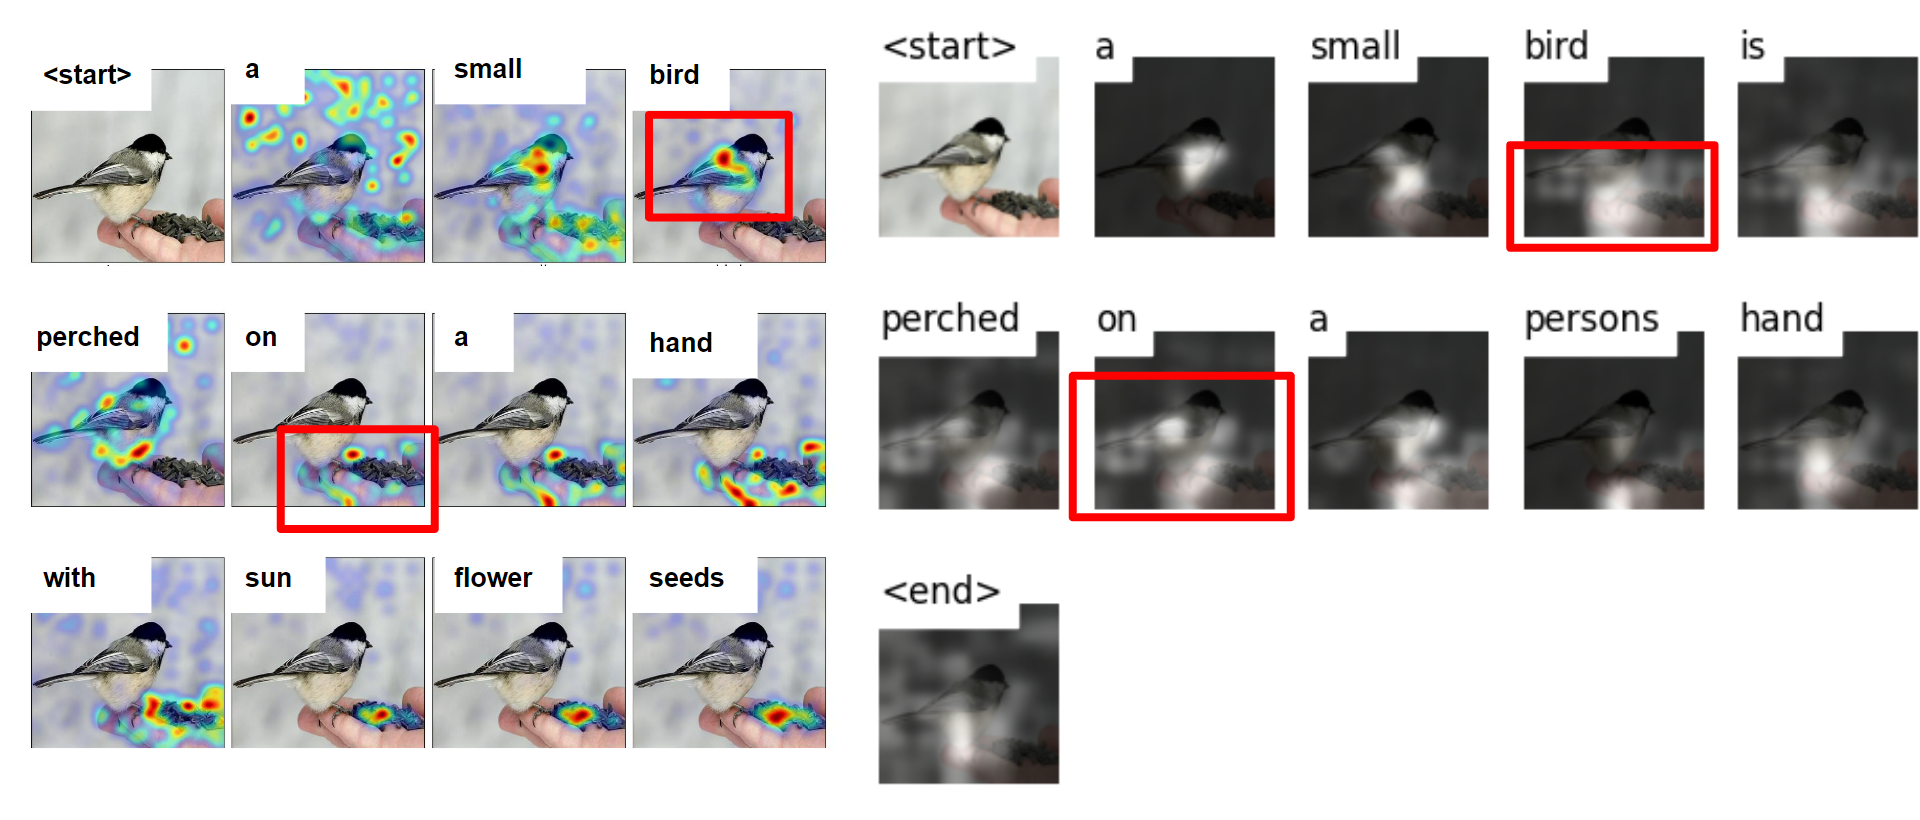
\includegraphics[width=1.1\linewidth]{../paper/images/bird_attention_comparison.png}
   \caption{Attention plots for both BLIP (on the left) and ResNet101 encoder/LSTM decoder (on the right).  We can see the differences in the models' capabilities when looking at the attentions for the tokens "bird" and "on". For "bird", BLIP's attention is focused mostly on the bird, while ResNet101 highlights both the bird and hand. For "on", BLIP's attention is targeted on areas of the hand where the bird could be standing, while ResNet101 highlights most of the bottom portion of the image.}
\label{fig:BLIP}
\end{figure*}

%-----------------------------------------------------------------------------------------------------------------------
\section{Experiments and Results}
%-----------------------------------------------------------------------------------------------------------------------
% NOTE -- we expect about 2 pages out of this section

%-----------------------------------------------------------------------------------------------------------------------
\subsection{Experiment I}
%-----------------------------------------------------------------------------------------------------------------------

\textbf{Setup} --We based our code on \cite{sagar2018}, which presents an image captioning model that employs an encoder-decoder architecture. The encoder was set to a pre-trained ResNet101, while the decoder was configured as an LSTM with attention. In this experiment, we focused on training the LSTM. The repository itself is 5 years old, which necessitated addressing compatibility issues throughout the entire lifecycle, from dataset loading to inference time, including the training process.

The first thing we tried was hyper-parameter tuning to get a benchmark and contrast the attention plots against those from the authors. We trained for 10 epochs using Google Colab, and plotted the loss (Figure \ref{fig:loss}) and accuracy (Figure \ref{fig:accuracy}) during training.

To compare and evaluate our model's performance, we also employed one of the state-of-the-art models for image captioning, as discussed earlier in the "Incorporating BLIP for Image Captioning" section (\ref{sec:blipapproach}). 

\textbf{Results} -- Our loss and accuracy plots reveal room for improvement, as an overfitting pattern emerges starting at epoch 4, with the training and validation curves diverging. Despite multiple trials on Google Colab, overcoming this pattern proved challenging due to the time required to reach epoch 4 (nearly 4 hours, with an approximate pace of 50 minutes per epoch). Moving forward, we plan to explore more hyper-parameter tuning and experiment with different regularization methods to enhance our model's performance. The BLEU-4 score for this model was 0.1148. For comparison, the best-performing state of the art model achieves a BLEU-4 score on COCO of 0.45.

On the other hand, when using the BLIP model for image captioning, we achieved a BLEU-4 score of 0.2734, which indicated a high performance. How the models differed in their attention became apparent when visualized on an image from the Flickr8k dataset (Figure \ref{fig:BLIP}). This further emphasizes the effectiveness of the BLIP framework in handling vision-language tasks and a better understanding of the reasons it peforms better than the alternate model.

\begin{figure}[!h]
\begin{center}
   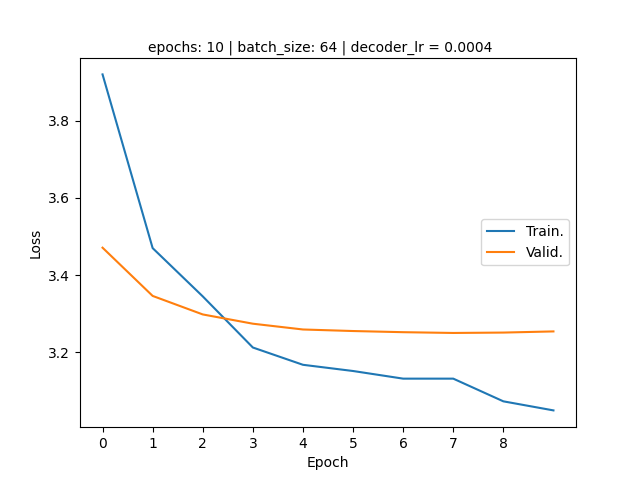
\includegraphics[width=0.8\linewidth]{../code/image-captioning-0/plots/learning_curves/loss-81d30535-1546-43f0-9477-e8e6fb14286a.png}
\end{center}
   \caption{Loss}
\label{fig:loss}
\end{figure}

\begin{figure}[!h]
\begin{center}
   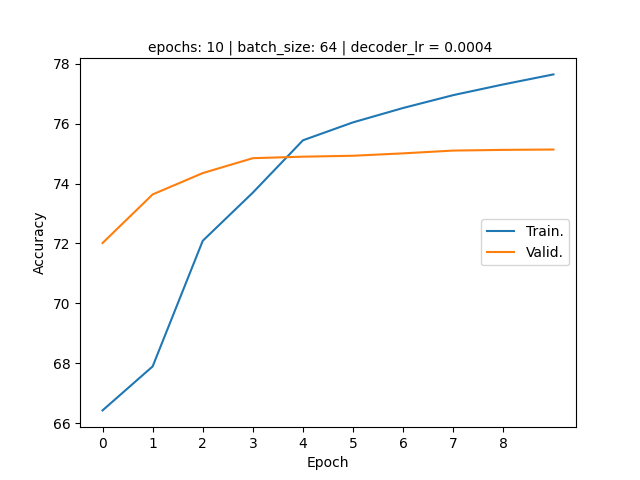
\includegraphics[width=0.8\linewidth]{../code/image-captioning-0/plots/learning_curves/accuracy-e934aac6-3f5b-437e-b6ce-b4505513e3d4.png}
\end{center}
   \caption{Top 5 Accuracy}
\label{fig:accuracy}
\end{figure}

%-----------------------------------------------------------------------------------------------------------------------
\subsection{Experiment II}
%-----------------------------------------------------------------------------------------------------------------------

\textbf{Setup} -- We used our above mentioned ResNet101 encoder-LSTM with attention (1 layer, 512 hidden dimension) decoder as the teacher model. The ResNet101 encoder is pre-trained on ImageNet but not fine-tuned. The LSTM decoder was trained on COCO 2014 TRAIN split (83,000 images) for 10 epochs using Adam optimization. Our student model is a ResNet50 encoder-LSTM with attention (1 layer, 256 hidden dimension). The student model was trained on COCO 2014 TEST split (41,000 images) for 2 epochs. When training the student model, we fine-tuned the CNN encoder as well as trained the LSTM decoder.\\

\textbf{Results} --As shown in Table \ref{tab:KDResult}, the student models with different temperatures for decoder KD achieved higher BLEU-4 scores than the baseline model. With a high temperature, the student model's performance is even better than the teacher model's performance. However, because the teacher model encoder was not fine-tuned, but the student model is fine-tuned by ground truth data in task loss, we hypothesize that the performance improvement comes from this uncontrolled factor. Thus, we removed the decoder KD loss and encoder KD loss in student 4 and student 5 respectively. The result is aligned with our hypothesis.

More experiments are needed to fully understand our results. For example, we could fine-tune the teacher model's encoder based on ground truth data and conduct KD again. Or we could assign independent weights for encoder loss and decoder loss, then do a more extensive and more granular hyper-parameter grid search, so as to understand how temperature and different components of the loss function impact performance improvement.


\begin{table*}[]
%\begin{sidewaystable}[ht]
    \centering
    \begin{tabular}{p{6cm}lllllrl}
        \toprule
        \textbf{Model} & \textbf{Training data} & \textbf{Loss} & \textbf{$\beta$} & \textbf{$T$} & \textbf{Epochs} & \textbf{BLEU-4} \\
        \midrule
        Teacher: ResNet101 - LSTM with attention (512 dimension) & COCO Train(83k) & Task & - & - & 10 & 0.1148   \\
        Student Baseline ResNet50 - LSTM with attention (256 dimension) & COCO Test(41k) & Task & - & - & 2 & 0.1039   \\
        Student1 ResNet50 - LSTM with attention (256 dimension) & COCO Test(41k) & Task+KD Encoder+ KD Decoder & 0.3 & 5 & 2 & 0.1098   \\
        Student2 ResNet50 - LSTM with attention (256 dimension) & COCO Test(41k) & Task+KD Encoder+ KD Decoder & 0.3  & 10 & 2 & 0.1121   \\
        Student3 ResNet50 - LSTM with attention (256 dimension) & COCO Test(41k) & Task+KD Encoder+ KD Decoder & 0.3  & 20 & 2 & 0.1207   \\
        Student4 ResNet50 - LSTM with attention (256 dimension) & COCO Test(41k) & Task+KD Encoder & 0.3  & - & 2 & 0.1312   \\
        Student5 ResNet50 - LSTM with attention (256 dimension) & COCO Test(41k) & Task+KD Decoder & 0.3  & 20 & 2 & 0.1104   \\

        \bottomrule
        \bottomrule
    \end{tabular}
    \caption{Knowledge Distillation Results}
    \label{tab:KDResult}
%\end{sidewaystable}
\end{table*}


%-----------------------------------------------------------------------------------------------------------------------
\section{Work Division}
%-----------------------------------------------------------------------------------------------------------------------

In the early stages of the project, all team members did independent research on possible image captioning topics. Once the team had settled on exploring model visualizations for image captioning, all members started independent work on exploring visualizations for different state of the art models. Next, Mouhcine, Chris, and Walker focused on generating attention plots for the Resnet/LSTM and BLIP models, while Xuan focused on exploring knowledge distillation. Once all the experiments were completed, all members focused on adding their observations to the report and organizing it into a neat and cohesive document. The breakdown of members' contribution can be seen in Table \ref {tab:contributions}.

\begin{table*}[]
\begin{center}
\begin{tabular}{|l|c|p{8cm}|}
\hline
Student Name & Contributed Aspects & Details \\
\hline\hline
Christopher Dugan & Model Visualizations and Report Synthesis & Generated attention plot visualizations. Edited report content and layout to be cohesive.  \\
Mouhcine Aitounejjar & Encoder-Decoder Model & Trained the encoder-decoder model, generated learning curves (loss/accuracy) and attention plots, fixed bugs that came up during data preparation, training and inference. Report editing.\\
Walker Stevens & BLIP Implementation & Researched literature of state-of-the-art models and funcionally how to implement them and extract the attention from them to use in visualization. Edited report.\\
Xuan Xu & Knoweldge Distillation & Initial literature review, brainstorming and resource collection for image captioning, attention visualization and knowledge distillation. Implememtation of knowledge distillation and experiments \\
\hline
\end{tabular}
\end{center}
\caption{Contributions of team members.}
\label{tab:contributions}
\end{table*}

\newpage
%-----------------------------------------------------------------------------------------------------------------------
% references
%-----------------------------------------------------------------------------------------------------------------------


{\small
\bibliographystyle{ieee_fullname}
\bibliography{paper}
}

\end{document}